\PassOptionsToPackage{table}{xcolor}
\documentclass[aspectratio=169,11pt]{beamer}

\usepackage[T1]{fontenc}
\usepackage{lmodern}
\usepackage{graphicx}
\usepackage{booktabs}
\usepackage{tikz}
\usetikzlibrary{positioning,arrows.meta}

\definecolor{RALblue}{HTML}{004878}
\definecolor{RALlight}{HTML}{E4EFF8}
\definecolor{TechSilicon}{HTML}{D9EAF7}
\definecolor{TechPixel}{HTML}{FCE4C5}
\definecolor{TechScint}{HTML}{E3F1D5}
\definecolor{TechHybrid}{HTML}{DDF2E6}
\definecolor{TechDose}{HTML}{E9DDF2}
\definecolor{TechNeutral}{HTML}{FFF2B2}
\definecolor{TechOther}{HTML}{E7E7E7}


\definecolor{newinst}{RGB}{180,30,30}
\definecolor{updatedinst}{RGB}{0,90,160}

\newcommand{\newi}[1]{\textcolor{newinst}{#1}}
\newcommand{\updi}[1]{\textcolor{updatedinst}{#1}}


\setbeamercolor{normal text}{fg=black,bg=white}
\setbeamercolor{structure}{fg=RALblue}
\setbeamercolor{frametitle}{fg=white,bg=RALblue}
\setbeamercolor{title}{fg=RALblue}
\setbeamercolor{subtitle}{fg=black!72}
\setbeamercolor{block title}{fg=white,bg=RALblue}
\setbeamercolor{block body}{fg=black,bg=RALlight}
\setbeamertemplate{navigation symbols}{}
\setbeamertemplate{itemize item}{\color{RALblue}$\blacktriangleright$}
\setbeamertemplate{itemize subitem}{\color{RALblue}$\bullet$}
\setbeamertemplate{footline}{%
  \leavevmode\hbox{%
  \begin{beamercolorbox}[wd=.82\paperwidth,ht=2.6ex,dp=1.1ex,leftskip=5mm]{author in head/foot}%
  \color{black!55}\scriptsize Space Radiation Monitor Survey 2026
  \end{beamercolorbox}%
  \begin{beamercolorbox}[wd=.18\paperwidth,ht=2.6ex,dp=1.1ex,rightskip=5mm plus1fil]{author in head/foot}%
  \color{black!55}\scriptsize\insertframenumber/\inserttotalframenumber
  \end{beamercolorbox}}}
\setbeamertemplate{headline}{%
  \leavevmode\hbox{%
  \begin{beamercolorbox}[wd=.5\paperwidth,ht=3.2ex,dp=1ex,leftskip=5mm]{author in head/foot}%
  
\includegraphics[height=2.4ex]{assets/UKRISTFCRALLogo.png}
  \end{beamercolorbox}%
  \begin{beamercolorbox}[wd=.5\paperwidth,ht=3.2ex,dp=1ex,rightskip=5mm plus1fil]{author in head/foot}%
  
\includegraphics[height=2.4ex]{assets/RALSpaceLogo.png}
  \end{beamercolorbox}}}

\newcommand{\source}[1]{\vfill{\tiny\color{black!55}Source: #1\par}}
\newcommand{\familycell}[2]{\cellcolor{#1}\strut #2}

\title{Space Radiation Monitors}
\subtitle{Heritage systems, emerging technologies and engineering gaps}
\author{Dr Ruth Bamford}
\institute{RAL Space}
\date{2026 review}

\begin{document}

% -----------------------------------------------------------------------------
\begin{frame}[plain]
\centering
\vspace{7mm}

\includegraphics[height=8mm]{assets/RALSpaceLogo.png}\par
\vspace{9mm}
{\fontsize{27}{31}\selectfont\bfseries\color{RALblue}Space Radiation Monitors\par}
\vspace{4mm}
{\Large Heritage systems, emerging technologies and engineering gaps\par}
\vspace{10mm}
{\large Dr Ruth Bamford\quad |\quad RAL Space\par}
\vfill
{\normalsize State-of-the-art review update, 2026\par}
\end{frame}

% -----------------------------------------------------------------------------
\begin{frame}{The review connects mature markets to emerging missions}
\large
The survey is organised around the engineering question: \textbf{what measurement capability fits the mission?}

\vspace{7mm}
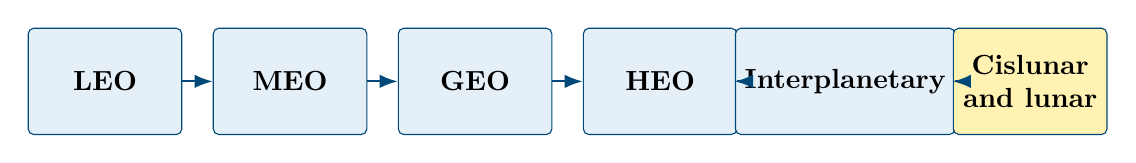
\begin{tikzpicture}[x=2.35cm,
  node/.style={draw=RALblue,rounded corners=2pt,minimum width=1.95cm,
  minimum height=1.35cm,align=center,fill=RALlight,font=\normalsize\bfseries},
  arr/.style={-{Latex[length=2.3mm]},thick,draw=RALblue}]
\node[node] (leo) at (0,0) {LEO};
\node[node] (meo) at (1,0) {MEO};
\node[node] (geo) at (2,0) {GEO};
\node[node] (heo) at (3,0) {HEO};
\node[node] (deep) at (4,0) {Interplanetary};
\node[node,fill=TechNeutral] (cis) at (5,0) {Cislunar\\and lunar};
\foreach \a/\b in {leo/meo,meo/geo,geo/heo,heo/deep,deep/cis} \draw[arr] (\a)--(\b);
\end{tikzpicture}

\vspace{7mm}
\begin{itemize}
\item The Kellett/SWIMMR material provides the heritage baseline.
\item Post-2023 developments are compared separately, using the same engineering fields.
\item Cislunar systems are included as an emerging market and a source of detector innovation.
\end{itemize}
\end{frame}

% -----------------------------------------------------------------------------
\begin{frame}{Mission domain changes the useful energy range}
\vspace{-2mm}
\begin{columns}[T,onlytextwidth]
\column{0.39\textwidth}
\begin{itemize}
\item \textbf{LEO:} trapped particles, SAA passages and atmospheric secondaries.
\item \textbf{MEO/GEO:} persistent energetic electrons, charging and solar-particle exposure.
\item \textbf{Beyond Earth:} SEP, GCR, heavy ions and locally generated secondaries.
\end{itemize}

\vspace{3mm}
{\color{RALblue}\bfseries Engineering consequence:}\par
No single energy range or detector architecture is optimal across every domain.

\column{0.58\textwidth}
\centering
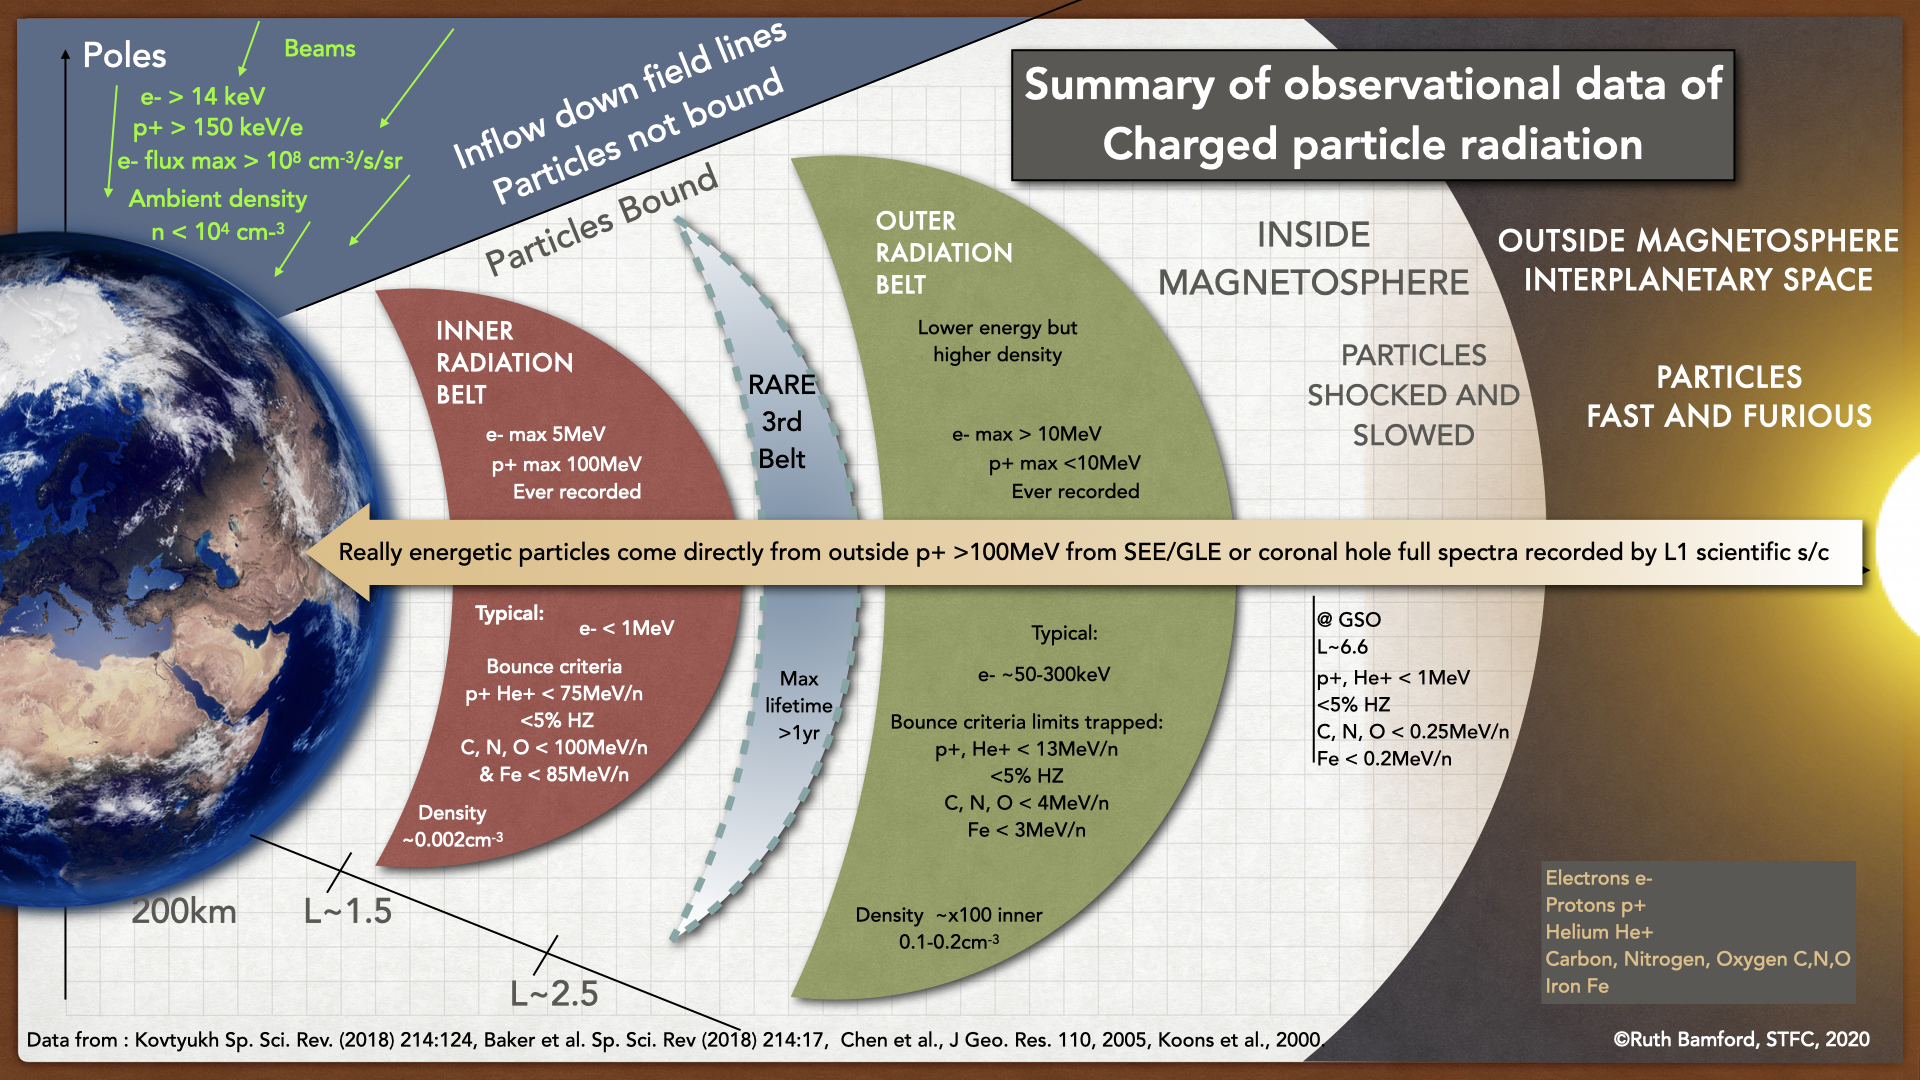
\includegraphics[width=\linewidth,height=0.59\textheight,keepaspectratio]{assets/Rad_Data_Summary_ImageSWIMMR.jpeg}
\end{columns}
\note{[Sources] Kovtyukh (2018); Baker et al. (2018); Koons et al. (2000).}
\end{frame}

% -----------------------------------------------------------------------------
\begin{frame}{Detector families occupy different parts of the trade space}
\scriptsize
\centering
\renewcommand{\arraystretch}{1.10}
\begin{tabular}{p{3.0cm}p{4.25cm}p{4.25cm}}
\toprule
\rowcolor{RALblue}
\color{white}\bfseries Family & \color{white}\bfseries Principal strength & \color{white}\bfseries Principal limitation\\
\midrule
\familycell{TechSilicon}{Silicon telescope} & Heritage and $\Delta E$--$E$ identification & Thickness, geometry and contamination\\
\familycell{TechPixel}{Pixel / Timepix} & Imaging, track classification and low SWaP & Stopping power and high-rate response\\
\familycell{TechScint}{Scintillator} & Active volume and high-energy stopping power & Species separation needs added information\\
\familycell{TechHybrid}{Hybrid Si--scintillator} & Tracking plus calorimetry over a broad range & Integration and cross-calibration complexity\\
\familycell{TechDose}{Dosimetry / TEPC} & Dose relevance and distributed monitoring & Limited spectral or directional information\\
\familycell{TechOther}{Magnetic / ToF} & Momentum, charge sign and composition & Mass, power and alignment\\
\bottomrule
\end{tabular}
\end{frame}

% -----------------------------------------------------------------------------
\begin{frame}{Heritage remains valuable ��but the instruments are not interchangeable}
\begin{columns}[T,onlytextwidth]
\column{0.50\textwidth}
\begin{block}{Operational heritage}
Silicon telescopes and multi-sensor suites provide defensible calibration, species separation and wide energy coverage.
\end{block}
\vspace{3mm}
\small
\begin{itemize}
\item SREM: multi-mission Earth-orbit and interplanetary heritage.
\item NGRM/RMU: compact operational electron and proton/ion sensor heads.
\item REPT: high-fidelity radiation-belt science.
\end{itemize}

\column{0.46\textwidth}
\centering
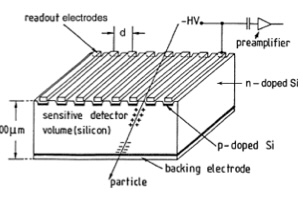
\includegraphics[width=0.72\linewidth]{assets/Silicon Solid-State Detectors (SSDs).jpeg}
\vspace{4mm}

\begin{block}{Miniaturised heritage}
Timepix-based instruments add track imaging and distributed sensing, with different limits on stopping power and flux.
\end{block}
\end{columns}
\end{frame}

% -----------------------------------------------------------------------------
\begin{frame}{Post-2023 work expands the architecture, not just the catalogue}
\begin{columns}[T,onlytextwidth]
\column{0.48\textwidth}
\centering
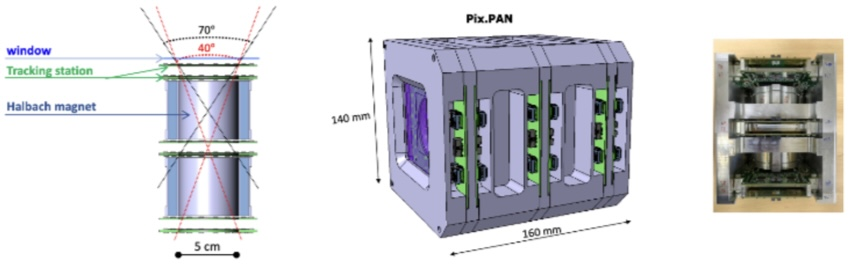
\includegraphics[width=\linewidth,height=0.56\textheight,keepaspectratio]{assets/LuPiX_PanPix.jpeg}

{\small Pix.PAN combines magnetic analysis, Timepix4 tracking and time-of-flight.}

\column{0.49\textwidth}
\begin{itemize}
\item \textbf{MATCH:} DSSD and BGO stack for lunar particles.
\item \textbf{PixPAN / NeuPix:} complementary charged- and neutral-particle concepts.
\item \textbf{IRADCAL:} compact scintillator/SiPM system for lunar albedo studies.
\item \textbf{HENON REPE:} directional electrons and protons from a 12U platform.
\end{itemize}

\vspace{1mm}
{\color{RALblue}\bfseries Common direction:} more particle information within constrained accommodation.
\end{columns}
\note{[Sources] Wang et al. (2024); LunPAN concept material; IRADCAL (2024); HENON REPE instrument paper (2026).}
\end{frame}

% -----------------------------------------------------------------------------
\begin{frame}{The remaining gaps are system-level gaps}
\scriptsize
\renewcommand{\arraystretch}{1.12}
\begin{tabular}{p{3.4cm}p{4.2cm}p{4.2cm}}
\toprule
\rowcolor{RALblue}
\color{white}\bfseries Capability & \color{white}\bfseries Present limitation & \color{white}\bfseries Opportunity\\
\midrule
Broad-range low-SWaP & Selected bands or model-dependent unfolding & Hybrid and stacked architectures\\
Extreme SEP response & Pile-up, saturation and telemetry demand & Adaptive processing and dual gain\\
Compact neutron measurement & Often a separate payload & Converter pixels and segmented scintillators\\
Directional measurements & Acceptance competes with angular information & Stacked pixels and multiple sensor heads\\
Cross-mission comparison & Mission-specific response and products & Open response matrices and calibration metadata\\
\bottomrule
\end{tabular}

\vspace{3mm}
\centering\normalsize
The priority is not a universal sensor; it is a \textbf{cross-calibrated family of instruments}.
\end{frame}

% -----------------------------------------------------------------------------
\begin{frame}{Select the measurement before selecting the detector}
\vspace{-3.5mm}
\begin{columns}[T,onlytextwidth]
\column{0.55\textwidth}
\normalsize
\begin{enumerate}
\setlength{\itemsep}{1mm}
\item Define the operational or scientific data product.
\item Specify species, energy, cadence and dynamic range.
\item Test contamination, saturation and angular response.
\item Confirm mass, power, telemetry, interfaces and heritage.
\item Require a traceable calibration and response matrix.
\end{enumerate}

\column{0.40\textwidth}
\begin{block}{Review conclusion}
\large
Pixel and hybrid systems broaden the available trade space, but they complement rather than automatically replace mature telescopes, calorimeters and dosimeters.
\end{block}

\vspace{3mm}
\centering
{\Large\bfseries\color{RALblue}Next step}\par
\vspace{2mm}
Complete the controlled comparison dataset and verify quantitative fields against primary sources.
\end{columns}
\end{frame}
%%%%%%%%%%%%%%%%%%%%%%%%%%%%%%%%%%%%%%%%%%%%%%%%%%%%%%%
% Previous Presentation

%%%%%%%%%%%%%%%%%%%%%%%%%%%%%%%%%%%%%%%%%%%%%%%%%%%%%%
\begin{frame}
	Previous Presentation Tables
\end{frame}

\begin{frame}{Orbit-Based View of Detector Developments}
\begin{itemize}
\item Instruments are grouped by measurement environment:
\begin{itemize}
    \item heritage LEO mapping / dosimetry systems
    \item MEO radiation-belt instruments
    \item cislunar / lunar-environment concepts
\end{itemize}
\item Highlighting used in the tables:
\begin{itemize}
    \item \textcolor{newinst}{Red}: not in the original baseline list
    \item \textcolor{updatedinst}{Blue}: baseline instrument with updated / changed performance or status
\end{itemize}
\end{itemize}
\end{frame}

%------------------------------------------------
\begin{frame}{LEO Instruments}
\scriptsize
\begin{tabular}{lcccc}
\toprule
Instrument & Type & Proton (MeV) & Mass & Status \\
\midrule
HMRM & Pixel Si & 0.6--500 & 52 g & flown \\
LUCID & Timepix array & $>$10 & 1.2 kg & flown \\
SATRAM & Timepix & ND & 172--380 g & flown \\
\updi{MIRAM} & Timepix3 + Si & 10--400 & $>$150 g & proposed / development \\
MERiT & SSD + APD & 7--100 & 1.13 kg & flown \\
\newi{RADMON (Aalto-1)} & Si + CsI & 10--80 & 360 g & flown \\
RISEPix & 2$\times$ Timepix stack & ND & $>$1 kg & flown \\
VZLUSAT-1 & Timepix & ND & ND & flown \\
\newi{ALTEA} & Si telescopes & ND & ND & flown \\
\newi{DosTel} & Si telescope & ND & ND & flown \\
TEPC & Gas proportional counter & ND & ND & flown \\
\newi{HEPD} & Si + scintillator & 30--200 & 43 kg & flown \\
\bottomrule
\end{tabular}

\vspace{0.3cm}
\footnotesize
LEO remains dominated by miniaturised, mapping, and dosimetry-oriented systems, especially Timepix-class detectors.
\end{frame}

%------------------------------------------------
\begin{frame}{MEO Instruments}
\scriptsize
\begin{tabular}{lcccc}
\toprule
Instrument & Type & Proton (MeV) & Mass & Status \\
\midrule
EMU & Si telescope & 15--100 & 3.5 kg & flown \\
\newi{Merlin} & Si + SURF & $>$40 & 1.7 kg & flown \\
\newi{CEDEX} & Si-based & ND & ND & flown \\
\newi{SREM (GIOVE-B)} & Multi-detector & 23--450 & 2.6 kg & flown \\
NGRM & Si (PSI) & 2--200 & 1.4 kg & flown \\
\newi{ICARE-NG} & Si coincidence & 27--292 & 2.8 kg & flown \\
CEASE3 & Si stacks & 2--150 & 4 kg & flown \\
\newi{CREDANCE} & Si detectors & ND & ND & flown \\
\newi{REPT} & Si stack & 17--200 & 13.4 kg & flown \\
\bottomrule
\end{tabular}

\vspace{0.3cm}
\footnotesize
MEO systems are primarily radiation-belt instruments with thicker silicon stacks and stronger spectral capability.
\end{frame}

%------------------------------------------------
\begin{frame}{Cislunar / Lunar-Orbit Instruments}
\scriptsize
\begin{tabular}{lcccc}
\toprule
Instrument & Type & Energy Range & Platform & Status \\
\midrule
\newi{CRaTER} & Si pairs + tissue-equivalent plastic & ND & LRO lunar orbit & flown \\
\newi{RADOM} & Mini dosimeter spectrometer & ND & Chandrayaan-1 lunar orbit & flown \\
\newi{MATCH} & DSSD + BGO & MeV range & Chang'E-7 & development \\
\newi{PixPAN} & Magnetic spectrometer + Timepix4 & 0.1--10 GeV & ESA LunPAN & concept \\
\newi{NeuPix} & Hybrid pixel detector & 10--100 MeV & ESA LunPAN & concept \\
\newi{IRADCAL} & Scintillator + SiPM & keV--100 MeV & 2U CubeSat concept & concept \\
\bottomrule
\end{tabular}

\vspace{0.3cm}
\footnotesize
Cislunar developments are increasingly hybrid, with explicit focus on lunar albedo particles, neutrons and gamma-rays.
\end{frame}

%------------------------------------------------
\begin{frame}{Comparison Across Orbit Regimes}
\small
\begin{tabular}{lccc}
\toprule
Orbit Regime & Dominant Detector Style & Main Driver & Typical Trend \\
\midrule
LEO & Pixel / compact Si / dosimetry & mapping, dose, variability & low SWaP \\
MEO & Silicon telescope stacks & trapped belts / spectra & higher fidelity \\
Cislunar & Hybrid pixel + scintillator + spectrometer & SEP, GCR, albedo, neutrons & multi-species capability \\
\bottomrule
\end{tabular}

\vspace{0.5cm}
\begin{itemize}
\item LEO: compact deployment and distributed monitoring
\item MEO: spectral discrimination in radiation belts
\item Cislunar: broad environment, secondaries from regolith, neutron sensitivity
\end{itemize}
\end{frame}

%------------------------------------------------
\begin{frame}{Physics Implications}
\small
\begin{itemize}
\item \textbf{LEO:} compact instruments are often sufficient for dose monitoring and spatial mapping
\item \textbf{MEO:} thicker detector stacks are required to resolve trapped particle populations
\item \textbf{Cislunar:} instrument requirements broaden to include:
\begin{itemize}
    \item SEP protons in the 10--100 MeV range
    \item GCR response at higher energies
    \item secondary neutrons and gamma-rays from regolith
\end{itemize}
\item This is why recent cislunar concepts are increasingly hybrid rather than pure silicon telescope or pure pixel systems
\end{itemize}
\end{frame}

%------------------------------------------------
\begin{frame}{Summary}
\begin{itemize}
\item Grouping instruments by orbit clarifies both technology choice and physics driver
\item \textcolor{newinst}{Red entries} identify instruments absent from the original baseline list
\item \textcolor{updatedinst}{Blue entries} identify baseline instruments whose status / performance has changed
\item LEO remains dominated by compact and pixel-based monitors
\item MEO remains the domain of silicon telescope systems
\item Cislunar developments show the clearest shift toward hybrid architectures
\end{itemize}
\end{frame}

\end{document}
